\documentclass[border=2mm,tikz]{standalone}
\usepackage{tikz}
\usetikzlibrary{datavisualization}
\usetikzlibrary{datavisualization.formats.functions}
\begin{document}
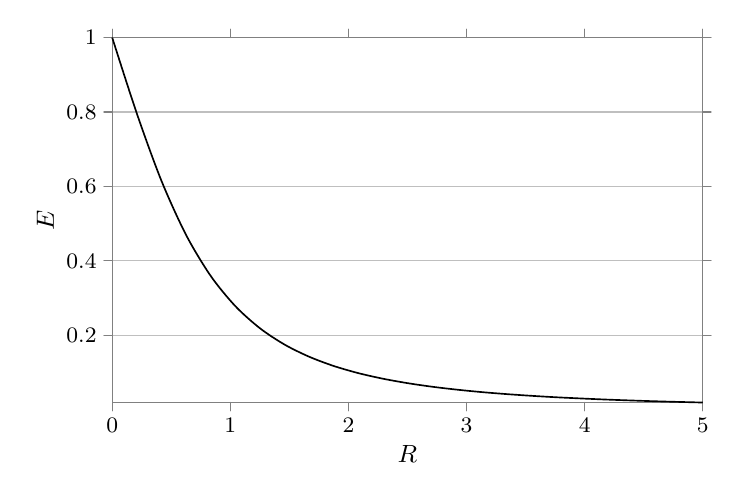
\begin{tikzpicture}
\datavisualization [scientific axes,
					y axis=grid,
                    y axis={label={$E$}},
                    x axis={label={$R$}},
                    visualize as smooth line,
                    scale = 1.5
                   ]

data [format=function]
{
  var x : interval [0:5];
  func y = 1 - ((\value x)/(sqrt(1 + \value x * \value x)));
};
\end{tikzpicture}
\end{document}